% Created 2026-07-18 Sat 13:18
% Intended LaTeX compiler: xelatex
\documentclass{article}
\usepackage{graphicx}
\usepackage{longtable}
\usepackage{wrapfig}
\usepackage{rotating}
\usepackage[normalem]{ulem}
\usepackage{capt-of}
\usepackage{hyperref}
\newcommand{\avg}[1]{\langle #1 \rangle}
\usepackage{amsmath}
\usepackage{amssymb}
\usepackage[thinc]{physics}
\usepackage{geometry}
\geometry{left=2.5cm,right=2.5cm,top=2.5cm,bottom=2.5cm}
\author{Soroush Seirani G.}
\date{\today}
\title{Avalanche's Progress Report}
\hypersetup{
 pdfauthor={Soroush Seirani G.},
 pdftitle={Avalanche's Progress Report},
 pdfkeywords={},
 pdfsubject={},
 pdfcreator={Emacs 30.2 (Org mode 9.7.11)}, 
 pdflang={English}}
\begin{document}

\maketitle
\section{Objectives}
\label{sec:orgad89c65}
\begin{itemize}
\item Fixing previous mistakes
\item Replicate two graphs from the paper
\end{itemize}
\section{Fixing Previous mistakes}
\label{sec:org6fac458}
In the previous report, I had included a faulty graph of the
simulation results. There were two problems with it:
\begin{enumerate}
\item The bins used to draw the histogram were of equal size while they
should've scaled logarithmically
\item The fitted power law didn't look like a straight line in the
log-log graph. That's because instead of fitting \(A x^{3/2}\) I had
absent mindedly fitted \(A x^{3/2} + B\). That's fixed now as well.
\end{enumerate}

I noticed there's no need to fit the power law because \(A\) can be
uniquely determined from the normalization condition:

\begin{align*}
  \sum_{n=1}^{\infty}P(n) &= 1\\
                  &= \sum_{n=1}^{\infty} A n^{-3/2}\\
                  &= A \sum_{n=1}^{\infty} n^{-3/2}\\
                  &= A \zeta(3/2) = 1\\
  \rightarrow A &= \frac{1}{\zeta(3/2)}
\end{align*}

Where \(\zeta\) is Reimann's zeta function.

You can see the result of \(1,000,000\) simulations and the exact solution below:
\begin{center}
\begin{center}
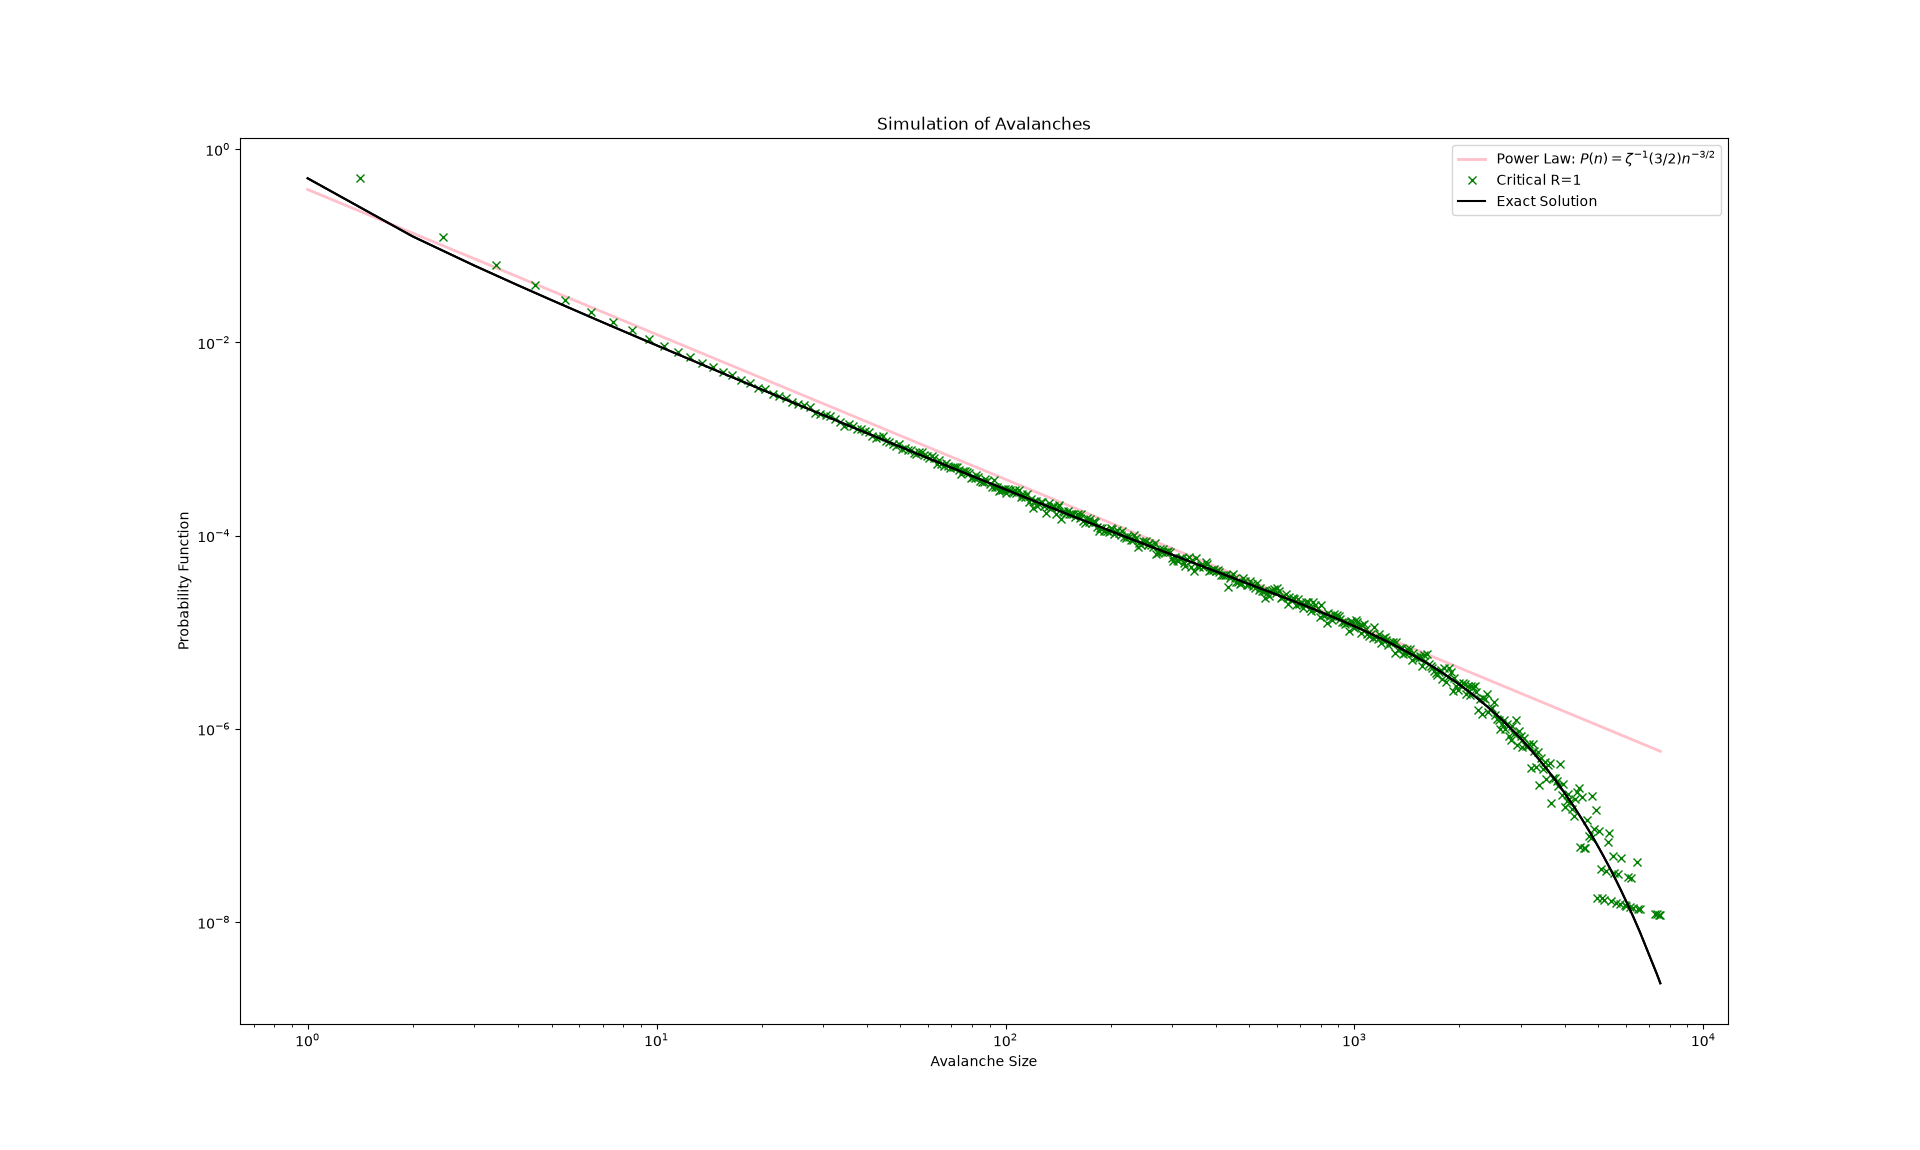
\includegraphics[width=.9\linewidth]{fig1.png}
\end{center}
\end{center}
\section{Replicating The First Two Graphs}
\label{sec:org5945e05}

The first graph is similar to the previous one but also includes the subcritical (\(R<1\)) and supercritical (\(R>1\)) cases:
\begin{center}
\begin{center}
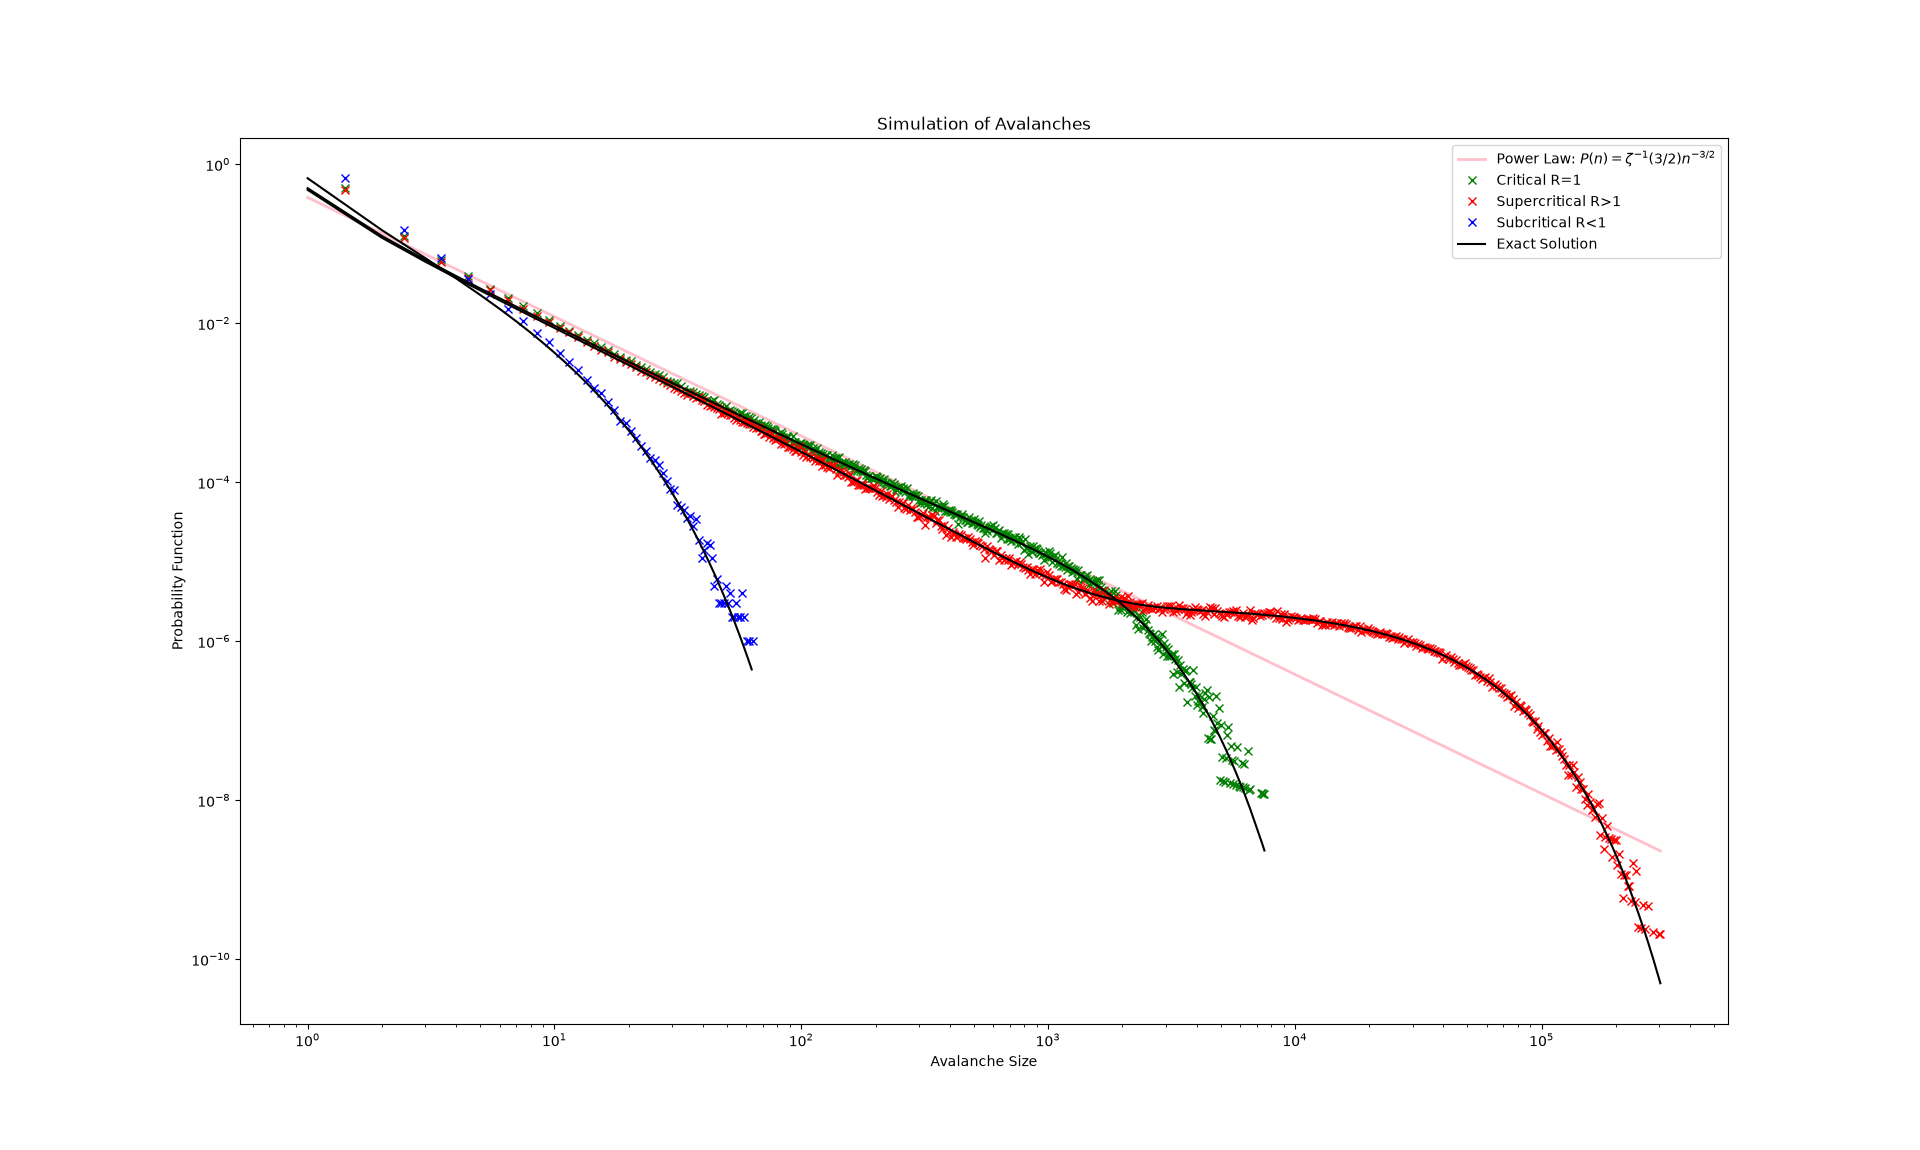
\includegraphics[width=.9\linewidth]{fig2.png}
\end{center}
\end{center}

The next graph is simply a time evolution of a system of neurons where you can see the number of active neurons at any point in time and observe the stabilizing of the system:
\begin{center}
\begin{center}
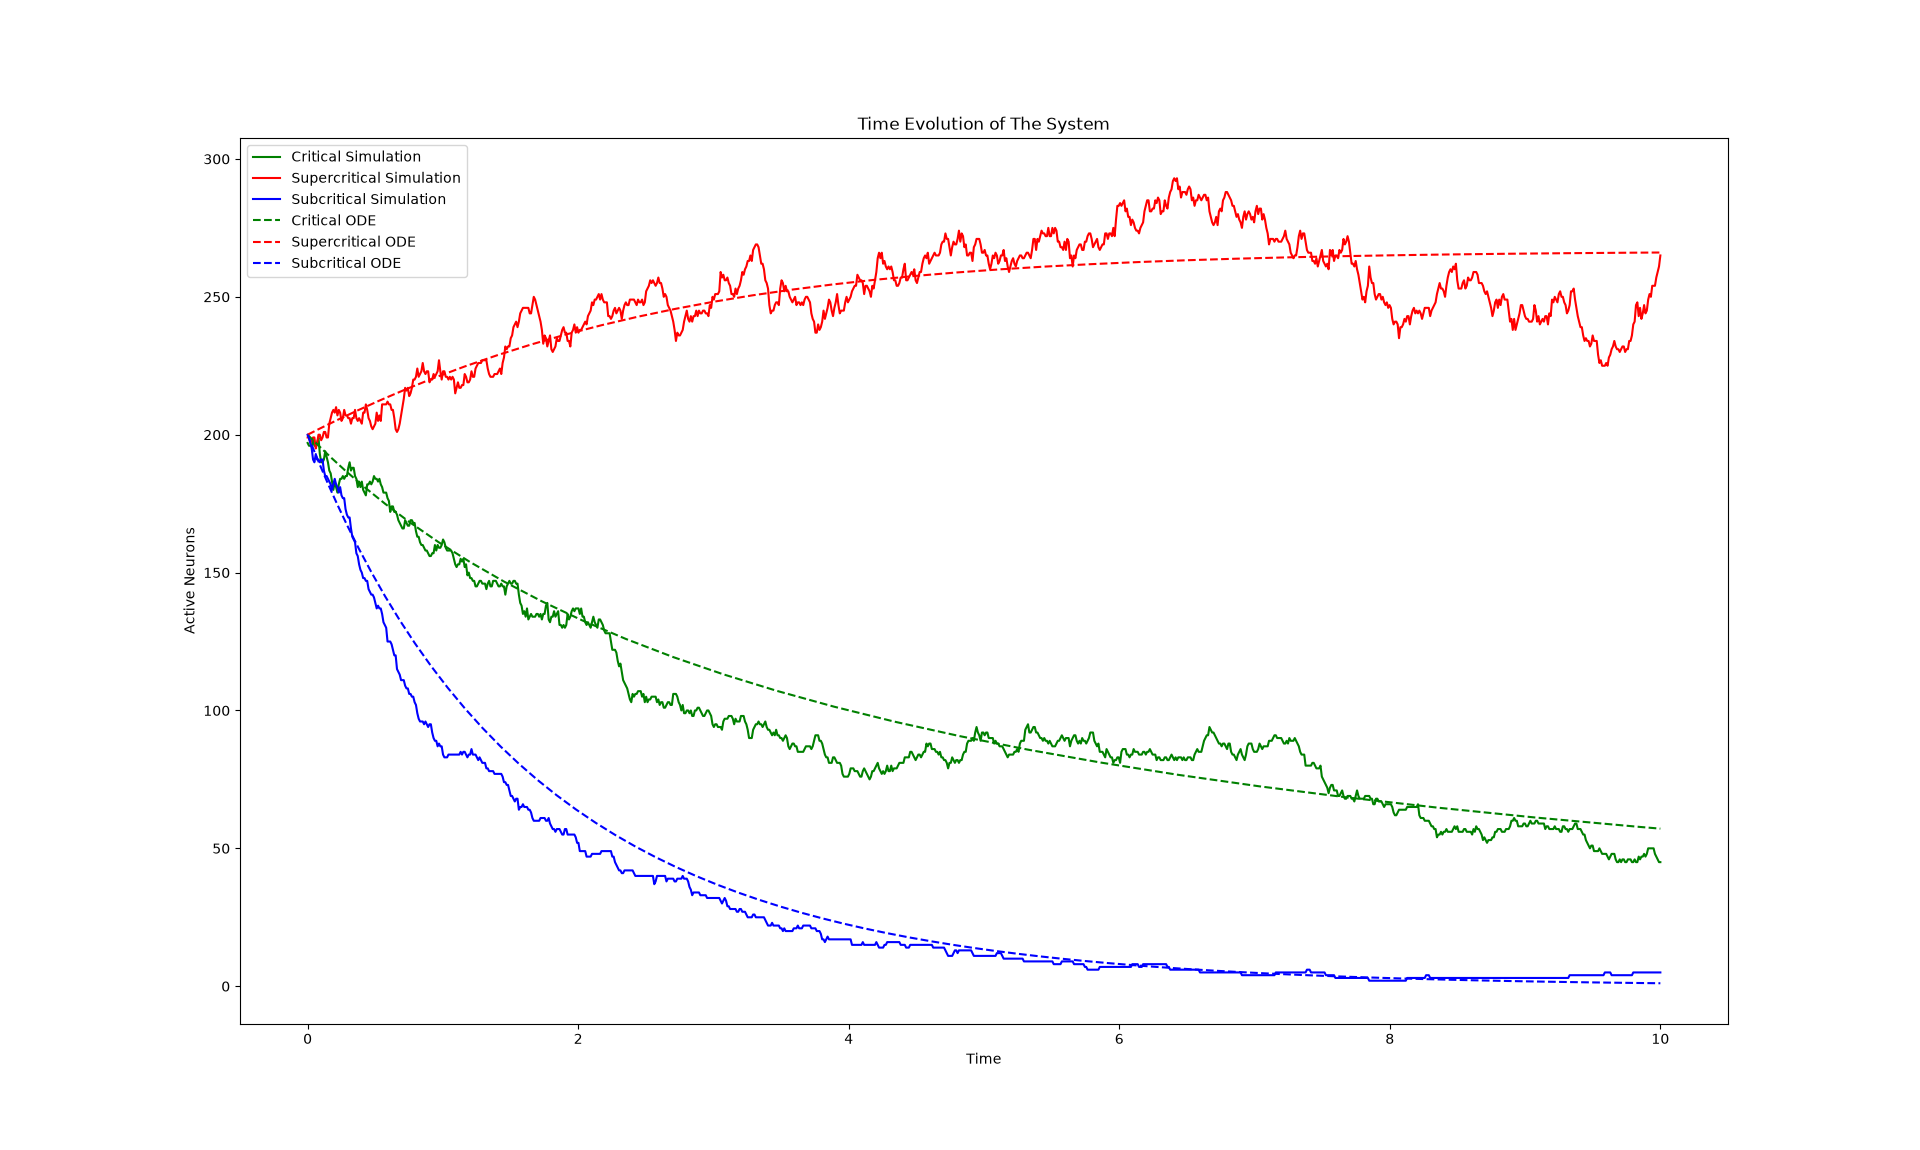
\includegraphics[width=.9\linewidth]{fig3.png}
\end{center}
\end{center}
\end{document}
